% PP-Article.tex for AEA last revised 22 June 2011
\documentclass[10pt, twocolumn, a4paper]{article}

%%%%%% NOTE FROM OVERLEAF: The mathtime package is no longer publicly available nor distributed. We recommend using a different font package e.g. mathptmx if you'd like to use a Times font.
\usepackage{mathptmx}
\usepackage{amsmath}
\usepackage[dutch]{babel}
\usepackage{subcaption}
\usepackage[width=.8\textwidth]{caption}
\usepackage{float}
\usepackage{booktabs}
\usepackage{multicol}
\usepackage{minted}
% If you have trouble with the mathtime package please see our technical support 
% document at: http://www.aeaweb.org/templates/technical_support.pdf
% You may remove the mathtime package if you can't get it working but your page
% count may be inaccurate as a result.
% \usepackage[cmbold]{mathtime}
\usepackage{xargs}                      % Use more than one optional parameter in a new commands
\usepackage[pdftex,dvipsnames]{xcolor}  % Coloured text etc.
% 
\usepackage{pdfpages}
\usepackage[colorinlistoftodos,prependcaption,textsize=tiny]{todonotes}
\newcommandx{\unsure}[2][1=]{\todo[linecolor=red,backgroundcolor=red!25,bordercolor=red,#1]{#2}}
\setlength{\marginparwidth}{2cm}
% Note: you may use either harvard or natbib (but not both) to provide a wider
% variety of citation commands than latex supports natively. See below.

% Uncomment the next line to use the natbib package with bibtex 
%\usepackage{natbib}
\usepackage{titlesec}

\titlespacing*\section{0pt}{12pt plus 4pt minus 2pt}{0pt plus 2pt minus 2pt}
\titlespacing*\subsection{0pt}{12pt plus 4pt minus 2pt}{0pt plus 2pt minus 2pt}
\titlespacing*\subsubsection{0pt}{12pt plus 4pt minus 2pt}{0pt plus 2pt minus 2pt}



% Uncomment the next line to use the harvard package with bibtex
%\usepackage[abbr]{harvard}

% This command determines the leading (vertical space between lines) in draft mode
% with 1.5 corresponding to "double" spacing.
\begin{document}

\title{Geavanceerde computerarchitectuur: Labo 01 \\ 
\large{Array omwisselen}}
\author{\textsc{Anton Danneels en Pieter Delobelle}}
\date{}
\maketitle

\section{Inleiding}
Het doel van dit labo is om een array om te draaien, zowel op de CPU alsook de GPU van de computer. 
Hierdoor moet een inzicht bekomen worden over het performantieverschil dat een GPU kan bieden ten opzichte van een CPU; en in welke situaties dit verschil naar boven komt.

Deze opdracht wordt ge\"implementeerd op een grafische kaart van NVIDEA, waarbij het \emph{CUDA}-framework gebruikt dient te worden. 

\section{Analyse}

\subsection{GPU}
Een GPU bestaat uit vele CUDA-cores, bedoeld om een \emph{single instruction multiple thread} (SIMT) architectuur te ondersteunen. Deze cores zijn verdeeld over een aantal \emph{stream multiprocessors} (SM), welke ook weer opgedeeld zijn in een aantal \emph{wraps}. Deze wraps bestaan typisch uit 32 threads, waardoor de blocksize idealiter een veelvoud van 32 is.

\subsection{CUDA}
Om de taken van de threads effici\"ent te kunnen verdelen, biedt CUDA een \emph{grid} aan. Dit grid bestaat uit blokken, die dus uitgevoerd worden door een SM. Binnen deze blokken kunnen threads ge\"identificeerd worden door een 1D, 2D of 3D set van indices. In ieder geval, de grootte $x \cdot y \cdot z$ kan niet groter zijn dan het aantal threads op een SM.

Om dit op te lossen, zijn blokken ook ge-indexed, waarbij een queue wordt aangelegd door de GPU. Om de algemene index te bepalen, wordt de volgende code gebruikt (voor 1 dimensie): 

\begin{minted}{C}
  int i = blockIdx.x * blockDim.x 
		+ threadIdx.x;
\end{minted}

\subsection{XOR-verwisseling}
Om de waarden te swappen, wordt gebruikt gemaakt van het \emph{XOR swapping algoritme}. Dit werkt als volgt:

\begin{minted}{C}
X = X XOR Y
Y = Y XOR X
X = X XOR Y
\end{minted}

\section{Oplossing}
Om de GPU en CPU te kunnen vergelijken, is de code om een array te swappen twee keer ge\"implementeerd: eenmaal voor de CPU met een traditionele for-lus en eenmaal voor de GPU, waarbij met variabele blocksize $n$.

Daarnaast is ook de lengte van de array variabel, waardoor de evaluatie over meerdere lengtes kan gebeuren. De code hiervoor is te vinden als bijlage.

\subsection{Swap op de CPU}
Voor de array om te wisselen op de CPU, itereren we tot het midden van de array, waarbij beide helften worden omgewisseld.

\subsection{Swap op de GPU}
De swap-operatie op de GPU is inhoudelijk gelijk, maar de lus is vervangen door bovenstaande functie om de indices te bepalen. 

\subsection{Vergelijking}
In figuur~\ref{blocksize} is de invloed van de grootte van de blocksize op de uitvoersnelheid weergegeven. Ter vergelijking is ook de tijd op de CPU weergegeven.

\begin{figure}
\centering
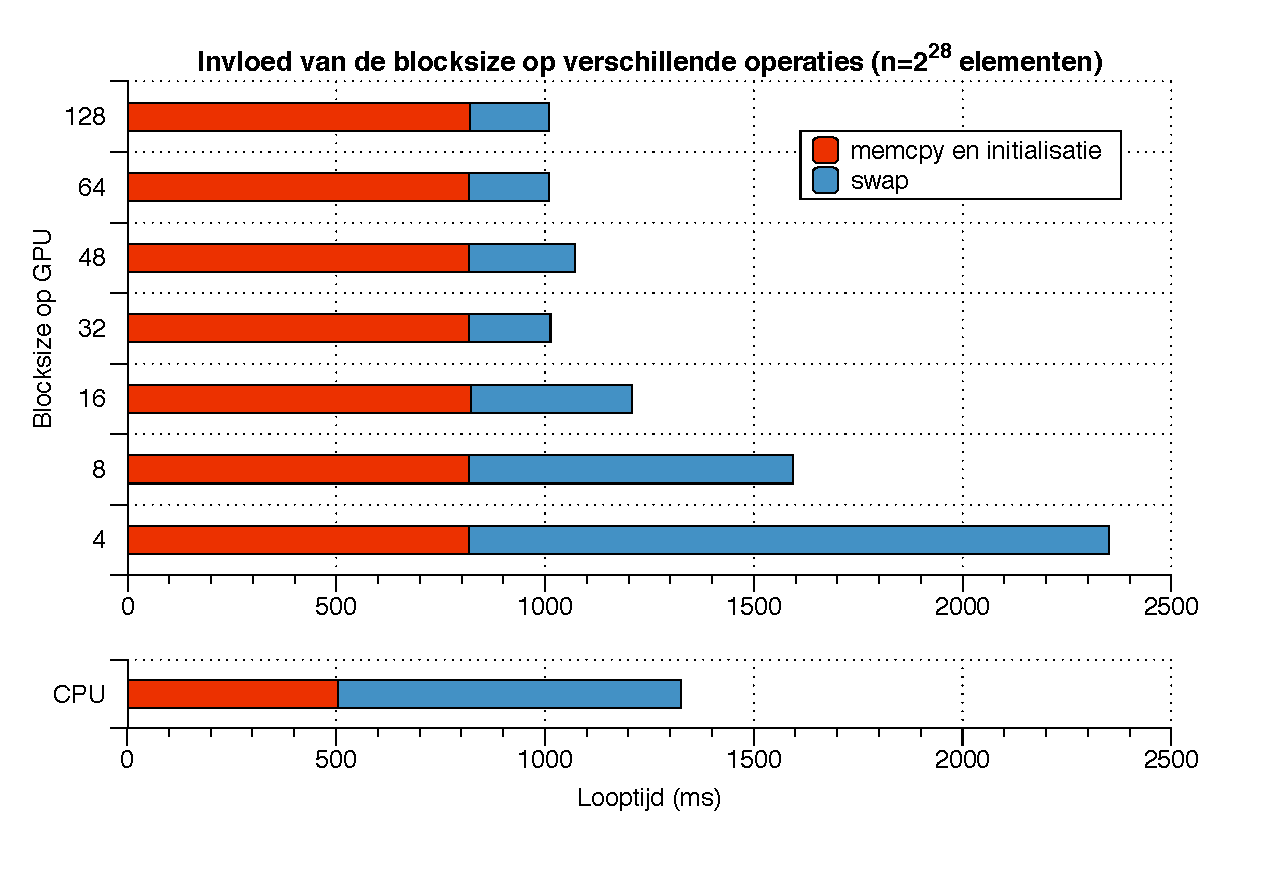
\includegraphics[width=0.5\textwidth]{blocksize.eps}
\caption{Invloed van de blocksize $n$.}
\label{blocksize}
\end{figure}

Uit de grafiek is duidelijk op te maken dat blocksizes $n$ die een veelvoud zijn van 32 een overduidelijk sneller zijn. Hoe beter de wraps benut worden---door dus veelvouden van 32 te kiezen, hoe beter de uitvoersnelheid is.

\begin{figure}
\centering
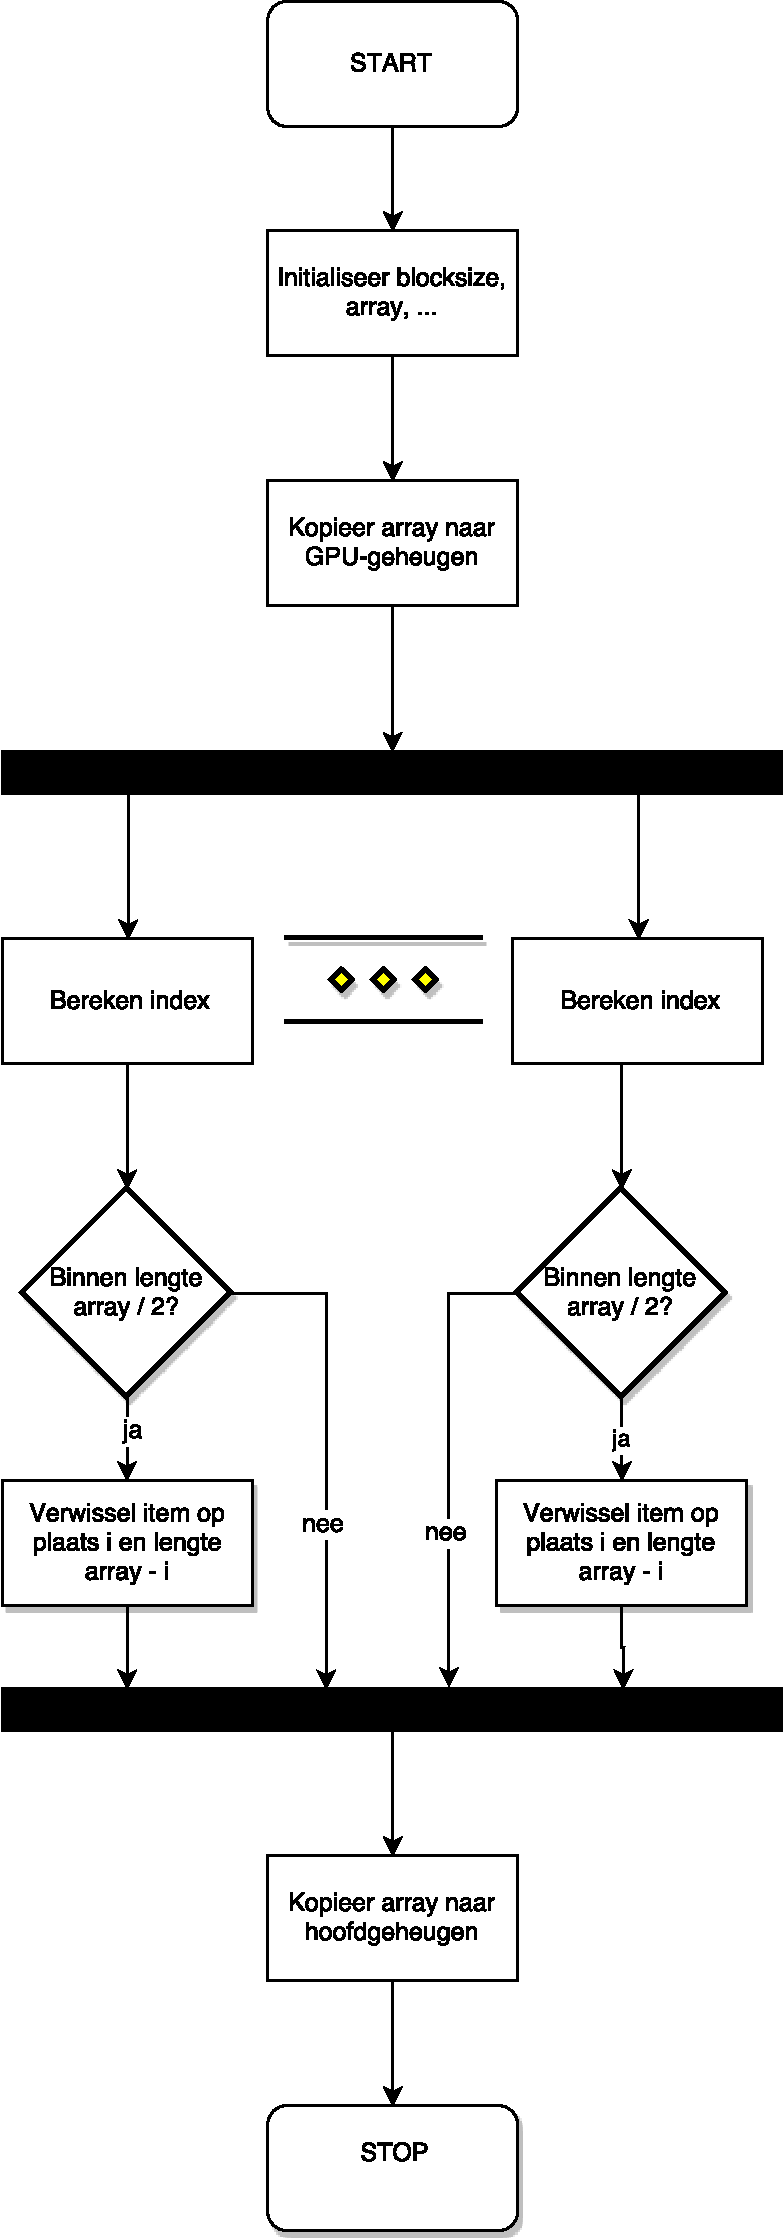
\includegraphics[width=0.4\textwidth]{flowgraph.pdf}
\caption{Flowchart van de code om de array te swappen op de GPU.}
\end{figure}

\section{Besluit}
beter/niet

\begin{figure*}
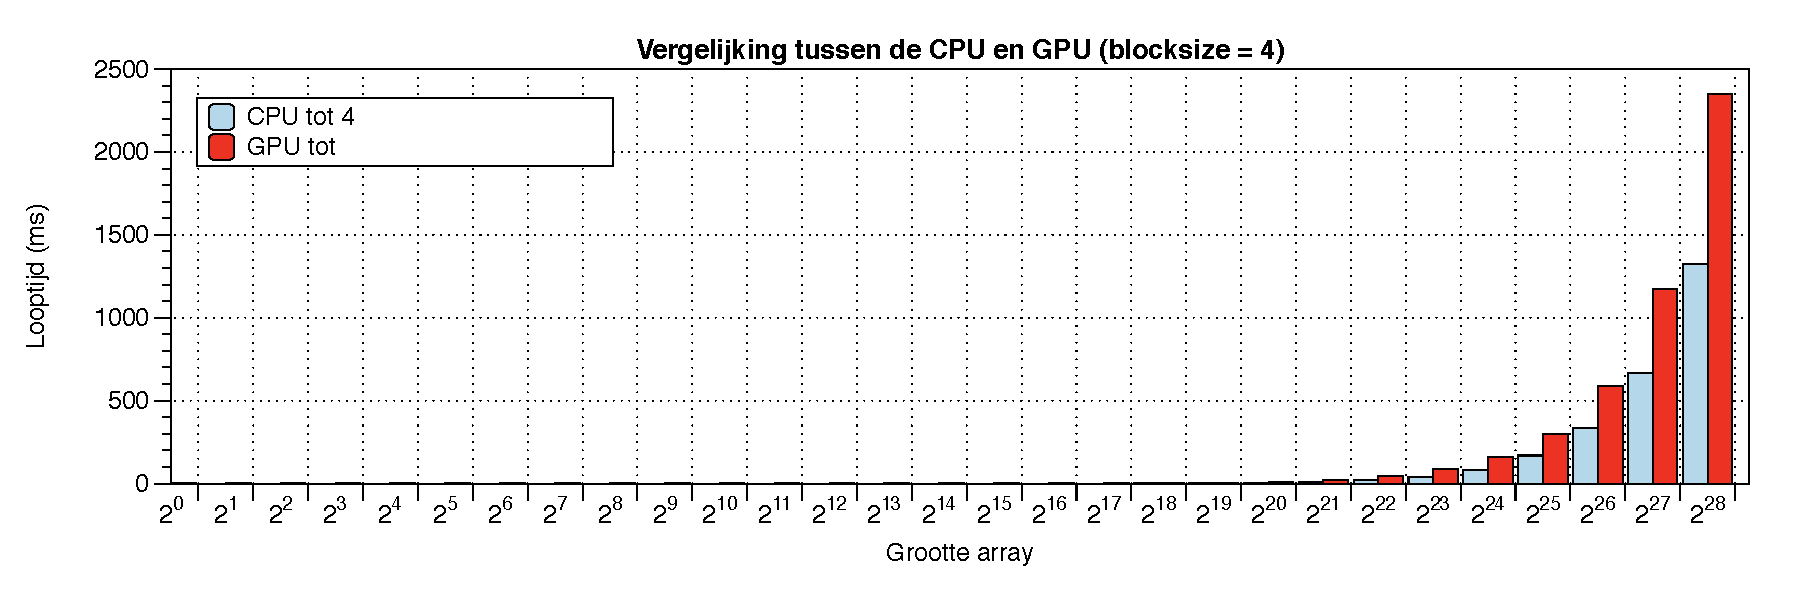
\includegraphics[width=\textwidth]{comp_4.eps}
\end{figure*}



\begin{minted}{console}
0000,0001,0002,0003,0004,0005,0006,0007,0008,0009 
0009,0008,0007,0006,0005,0004,0003,0002,0001,0000 
Operation in 0 ms
\end{minted}

\onecolumn

\appendix
\inputminted[tabsize=4,obeytabs]{c}{main.c}

% The appendix command is issued once, prior to all appendices, if any.
%\appendix
\end{document}

